 \documentclass[final]{article}


\usepackage{APS360}
\usepackage[utf8]{inputenc} % allow utf-8 input
\usepackage[T1]{fontenc}    % use 8-bit T1 fonts
\usepackage{hyperref}       % hyperlinks
\usepackage{url}            % simple URL typesetting
\usepackage{booktabs}       % professional-quality tables
\usepackage{amsfonts}       % blackboard math symbols
\usepackage{nicefrac}       % compact symbols for 1/2, etc.
\usepackage{microtype}      % microtypography
\usepackage{xcolor}         % colors
\usepackage{graphicx}
 
\title{Detecting Medical Misinformation in Social Media and Headlines}

\author{%
  Sissi Li \\
  1008884566, sissi.li@mail.utoronto.ca\\
  \url{https://colab.research.google.com/drive/1gTw8tCjCoNoS-6Xt-sN4I62u_1DDmRV9\\}
}

\begin{document}

\maketitle

\vspace{-0.5in}

\section*{Introduction}
Medical misinformation spreads rapidly through social media and threatens public health by deterring people from seeking appropriate medical care. This project aims to build an automated deep learning model to classify short-form medical text as containing misinformation or not. Recurrent Neural Networks (RNNs) are appropriate for this task since they can capture the sequential dependencies and contextual significance of words in a sentence, allowing the model to learn linguistic patterns that are missed by traditional keyword matching algorithms. To ensure the system is effective, the model’s success will be measured by evaluation metrics including Recall, Precision, F1-Score, Accuracy, and Loss \cite{padalko2024novel}.

\section*{Illustration}
\begin{figure}[htbp]
    \centering
    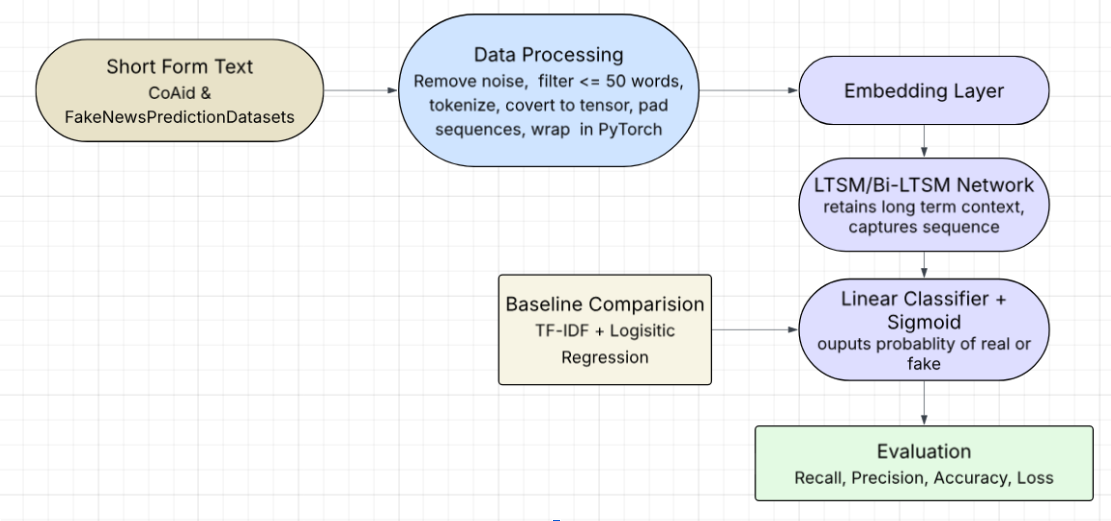
\includegraphics[width=0.8\textwidth]{Model_Illustration.png}
    \caption{Illustration of the overall pipeline for the project.}
    \label{fig:my_image_label}
\end{figure}

\section*{Background \& Related Work}
Research into medical misinformation analyzes how digital misinformation spreads. In their study of COVID-19 media trends, Zhao et al. (2021) define medical misinformation as false health claims that are not supported by scientific evidence \cite{chen2021characteristics}. Zubiaga et al. (2018) similarly note in their survey that these rumours are unverified at the time of posting \cite{zubiaga2018detection}. Furthermore, Liu et al. (2019) demonstrated that linguistic patterns in misleading claims rely on personal experience and sensationalized clickbait to maximize propagation \cite{liu2019analysis}. Learning these patterns is crucial for training the neural network to accurately detect misleading text. 

In terms of tested models, deep learning models have improved in classification accuracy in natural language processing tasks. For instance, Nasir et al. (2021) demonstrated that deep learning methods using Long Short-Term Memory (LSTM) networks can capture temporal dependencies \cite{lokhande2023fake}. This method achieved higher detection accuracy across multiple fake news datasets compared to non-hybrid baselines. Recent advancements have focused on optimizing RNN architectures to capture contextual nuances better. Syed et al. (2023) introduced the use of Bidirectional LSTMs (BiLSTM) and an attention mechanism \cite{padalko2024novel}. This successfully manages long-term linguistic dependencies and focuses on the specific words within a text that indicate deception. By leveraging these established LSTM-based methods, the proposed model aims to accurately classify short-form medical claims by identifying the underlying sequential structures of misinformation.
\section*{Data Processing}
The datasets CoAID and FakeNewsPrediction will be used \cite{arashnic_covid19_fakenews}\cite{kumar_fake_news}, with the main focus on the social media and headline subsets for short-form medical claims. To process the data, the following steps will be taken: 

1. Only short-form text (50 words or less) will be extracted to align with the memory retention strengths of an RNN. 
URLs, user handles (@), hashtags, stopwords, and special characters will be removed to reduce noise in the dataset. All text will be converted to lowercase. 

2. Tokenize the cleaned text and convert the textual data into a numerical tensor format compatible with PyTorch.

3. Pad all input sequences to a fixed length to ensure uniform matrix dimensions for efficient batch processing.

4. Wrapping the processed data into PyTorch Dataset and DataLoader objects.
\section*{Architecture}
The model will use an RNN-LSTM network where the Embedding Layer of the network will first map the tokenized vocabulary of the short-form medical claims into dense vector representations, which are then fed into a Long Short-Term Memory (LSTM) or Bidirectional LSTM (Bi-LSTM) network \cite{10370534}. Unlike standard RNNs, LSTMs mitigate the vanishing gradient problem and allow the model to maintain an internal memory state to retain long-term contextual information. Finally, the extracted sequence passes through a linear classifier and uses a Sigmoid activation function to output the final prediction of whether the text is real or fake.
\section*{Baseline Model}
This neural network will be compared against a simple baseline model using Logistic Regression and TF-IDF vectorization. This baseline model works by counting how often specific keywords appear in a post, but ignores word order and context \cite{ekoh_sentiment_baseline}. By comparing the LSTM model to a simple keyword counter, it demonstrates whether understanding the full context of a sentence is necessary to catch fake news. Additionally, this baseline will show exactly which specific words the model flags most often as medical misinformation. 
\section*{Ethical Considerations}
Misinformation detection systems introduce ethical challenges such as misclassification harm, algorithmic bias, and data privacy. Falsely labelling accurate medical advice as "fake" can censor valid health discussions. This can lead to backlash from social media users who feel their posts are being unfairly censored \cite{9253994}. Failing to detect harmful misinformation directly deters families from seeking medical treatment. Beyond classification errors, there is a risk of algorithmic bias if the training data overrepresents specific demographics. Finally, because the model processes public social media interactions, it is important to protect user privacy. To mitigate these concerns, the project will utilize diverse training data to ensure balanced and accurate detection of misinformation to successfully protect families from dangerous health decisions without compromising user privacy.

\textbf{Link to GitHub:} https://github.com/sissi820li/APS360/tree/main/MisinformationDetectionProject

\newpage
\cite{padalko2024novel}
\cite{chen2021characteristics}
\cite{zubiaga2018detection}
\cite{liu2019analysis}
\cite{lokhande2023fake}
\cite{arashnic_covid19_fakenews}
\cite{kumar_fake_news}
\cite{10370534}
\cite{ekoh_sentiment_baseline}
\cite{9253994}
\bibliographystyle{IEEEtran}
\bibliography{references}
\end{document}